\DiaryEntry{Max-Flow Algorithms, Further Topics II}{2020-07-01}{Algorithms}

We next consider the case of a flow network and investigate what happens to the max-flow when we add some high-capacity edges to the network.

As before, we consider a random graph from the Erdős–Rényi model. In addition, we have $n_a$ high-capacity edges which we place between two randomly selected vertices (this allows that a high-capacity edge is placed between the same vertex, thereby rendering the edge useless). We have several parameters to play with: The number of vertices $n_v$ of the graph, the probability $p$ of an edge between two nodes, the number of high-capacity edges $n_a$ and their capacity $c_a$.

One effective use of these high-capacity links is to directly connect the source vertex with the target vertex via all $n_a$ high-capacity links in parallel. In this case, we obtain a flow gain of $n_a \times c_a$. I'm not sure whether there is a better way to use the links. However, the probability that one such edge is chosen (by the random placement strategy above) is very low, namely

\bee
\frac{n_a}{n_v^2}
\eee

\paragraph{Simulation Results.} We consider Erdős–Rényi graph with $n_v=100$ and $p=0.1$. The capacity of each edge is $1$, and we add $n_a=10$ high-capacity edges with an capacity of $c_a = 10$. The following Figure shows the capacity histogram of the original capacity and the capacity with the high-capacity edges of $50000$ such simulations.

\begin{figure}[H]
\centering
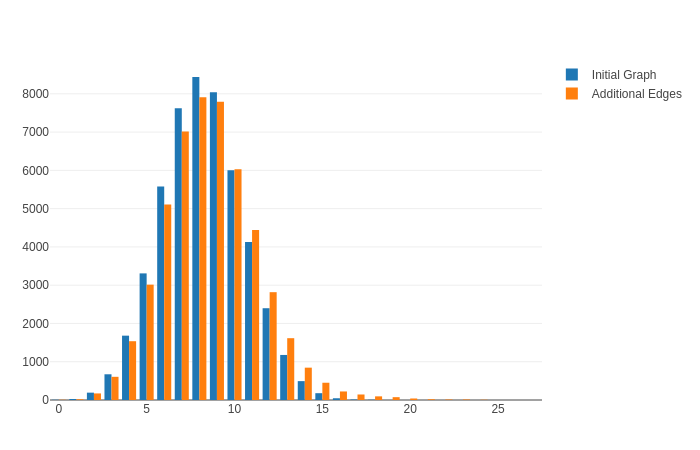
\includegraphics[scale=0.55]{images/max_flow_05_01.png}
\end{figure}

There are too few additional edges for any (significant) impact; the mean capacity increases from $8.2$ to $8.6$ and the histogram does not show much difference. If we increase the number of high-capacity edges to $n_a=100$, we obtain the following histogram.

\begin{figure}[H]
\centering
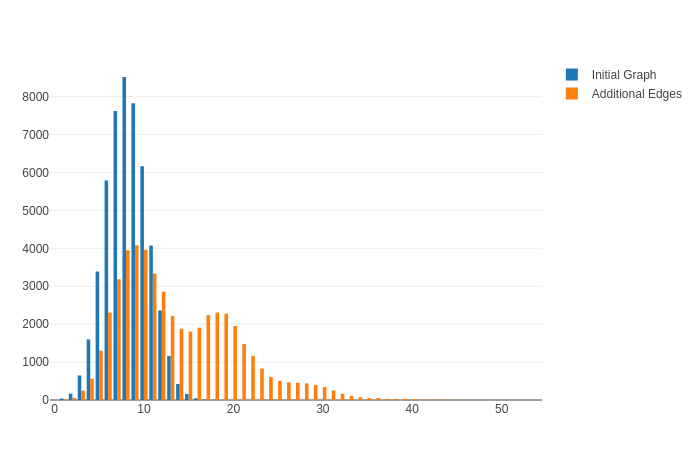
\includegraphics[scale=0.55]{images/max_flow_05_02.png}
\end{figure}

Interestingly, it seems that there are two networks: Once containing of the ``normal'' edges, the other one containing of the high-capacity links. The mean capacity increases from $8.2$ to $13.8$. The effect is even stronger for $n_a = 1000$ high-capacity edges as the following histogram shows. The mean has increased to $86$, one order of magnitude higher.

\begin{figure}[H]
\centering
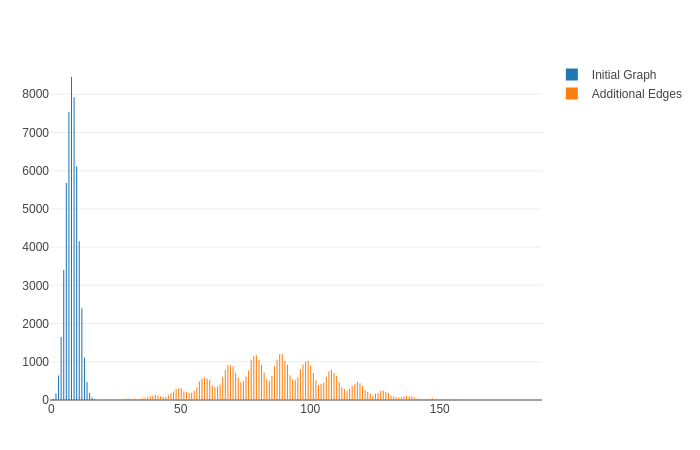
\includegraphics[scale=0.55]{images/max_flow_05_03.png}
\end{figure}

If we increase the number of ``normal'' edges by using $p=0.5$, we get the same picture. Adding $n_a=10$ high-capacity edges yields higher mean capacities (as there are more edges), but the high-capacity edges are too few to have an impact. If we add $n_a=100$ high-capacity egdes, we get the following histogram, with the mean increasing from $46.7$ to $52.9$.

\begin{figure}[H]
\centering
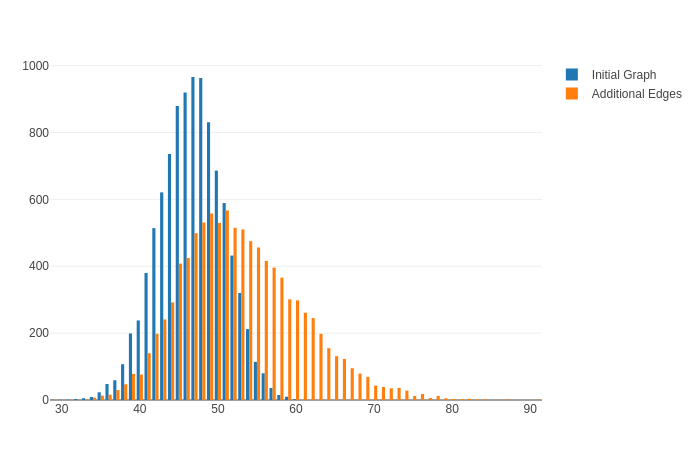
\includegraphics[scale=0.55]{images/max_flow_05_04.png}
\end{figure}

Adding $n_a=1000$ high-capacity edges yields the following hisogram. The mean capacity has only increased to $123$ (a factor of $3$), this is due to the fact, that the original graph had already more edges and therefore a higher capacity.

\begin{figure}[H]
\centering
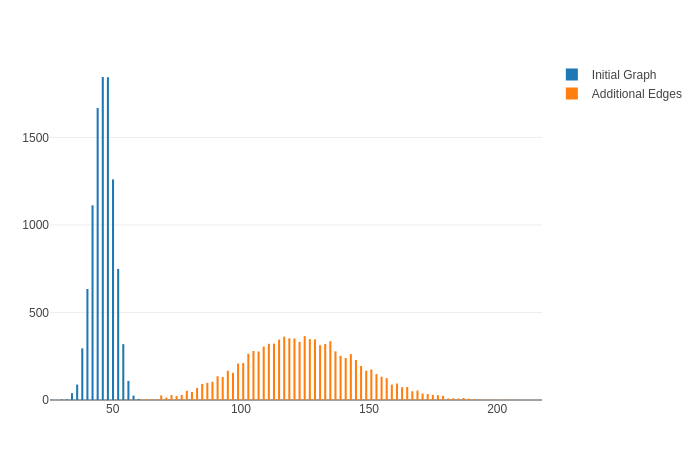
\includegraphics[scale=0.55]{images/max_flow_05_05.png}
\end{figure}

Increasing the number of edges in the original graph even more by setting $p=0.9$, the capacity difference due to $n_a=1000$ high-capacity edges is even smaller. In this case, the mean capacity increases from $87.4$ to $160$, which is a factor of $2$.

%%% Local Variables:
%%% mode: latex
%%% TeX-master: "journal"
%%% End:
